\chapter{能量在日常生活中}\label{ch:g5:everyday-energy}

一个上紧发条的玩具在地板上飞快地跑动，慢下来，然后停住——直到
你再次给它上紧发条。手电筒的\omterm{def:g3:first-electric-circuit:battery}{电池}用久了，\omterm{def:g4:light-straight-lines:ray}{光线}就变暗。你自己
在午饭前也会没了力气。凡是在运动、发光、发声或发热的东西，
似乎都在消耗着什么。物理学给这种“什么”起了一个名字，
它可能是整本书中最重要的一个词，
那就是\omterm{def:g5:everyday-energy:energy}{能量}。

\section{使事物运转的“东西”}

\begin{definition}[能量]\label{def:g5:everyday-energy:energy}
\emph{能量}\index{能量}是使事物发生变化所需的东西：
使物体运动、举起物体、使它发光、使它发热、使它发出\omterm{def:g3:sound-around-us:sound}{声音}。
没有能量被消耗，任何东西都不会运动、发光或生长——而且，
正在消耗能量的那个东西，自身必须先具有能量，
才能去消耗。
\end{definition}

\begin{definition}[能量储存]\label{def:g5:everyday-energy:store}
\emph{能量储存}\index{能量储存}是指储存着可供使用的\omterm{def:g5:everyday-energy:energy}{能量}的任何东西。
日常生活中主要的\omterm{def:g5:everyday-energy:energy}{能量}储存有：\emph{食物}（人体的燃料）、
\emph{燃料}（如木材和汽油）、充好电的\emph{\omterm{def:g3:first-electric-circuit:battery}{电池}}、
上紧的\emph{弹簧}，以及大坝后面\emph{高处}储存的水 ——
还有炽热的\emph{太阳}，
它整日向万物倾泻\omterm{def:g5:everyday-energy:energy}{能量}，而且不收费。
\end{definition}

\begin{example}[找出储存]\label{ex:g5:everyday-energy:spot}
每一个在运动的东西背后都有\omterm{def:g5:everyday-energy:store}{能量储存}。跑动的玩具：它上紧的弹簧。
手电筒：它的\omterm{def:g3:first-electric-circuit:battery}{电池}。汽车：油箱里的燃料。
你：你的早餐。帆船：风中流动的\omterm{def:g2:air-around-us:air}{空气}。
当储存耗尽——弹簧松开，\omterm{def:g3:first-electric-circuit:battery}{电池}没电，
油箱见底，午饭时间临近——运动就停止了。
\end{example}

\begin{remark}[没有供给，就没有运动]\label{rem:g5:everyday-energy:nofree}
几个世纪以来，发明家们一直在追寻无需任何\omterm{def:g5:everyday-energy:energy}{能量}就能永远运转的机器：
能自行转动的轮子，永远不需要上紧的钟表。
然而每一个都失败了。它们的失败揭示了物理学最深刻的教训之一：
\omterm{def:g5:everyday-energy:energy}{能量}绝不会凭空产生。
任何在运转的东西都在获得供给——找到\omterm{def:g5:everyday-energy:store}{能量储存}，
你就理解了这台机器。
\end{remark}

\section{能量的形式会变化}

\begin{example}[能量的形式]\label{ex:g5:everyday-energy:forms}
\omterm{def:g5:everyday-energy:energy}{能量}以不同的形式表现出来：滚动的球和吹动的风中有\emph{动能}；
从灯和太阳倾泻而下的是\emph{光能}；
一切温热的物体中有\emph{热能}；
沿导线传输的是\emph{电能}；
静静地储存在食物、燃料、弹簧和被举高的物体中的，是\emph{储存的\omterm{def:g5:everyday-energy:energy}{能量}}；
同一种东西，多种形式。
\end{example}

\begin{proposition}[能量链]\label{prop:g5:everyday-energy:chain}
每当有事情发生，\omterm{def:g5:everyday-energy:energy}{能量}就从某个储存中取出并传递下去，
通常在途中改变形式。\omterm{def:g5:everyday-energy:energy}{能量}绝不会凭空产生，
也从来不会真正消失——机器所“用掉”的\omterm{def:g5:everyday-energy:energy}{能量}，
只是被传递了出去，最终大多以柔和的热量形式
散布到周围环境中。
\end{proposition}

\begin{method}[阅读能量链]\label{met:g5:everyday-energy:read}
要理解任何装置，请追踪它的\omterm{def:g5:everyday-energy:energy}{能量}链：
\begin{enumerate}
  \item 找出\omterm{def:g5:everyday-energy:energy}{能量}的\emph{储存}来源；
  \item 找出\emph{转换器}——也就是\omterm{def:g5:everyday-energy:energy}{能量}
        在此改变形式的部件；
  \item 说出输出的各种形式——有用的那一种，以及
        随之泄漏的热量。
\end{enumerate}
以手电筒为例：\omterm{def:g3:first-electric-circuit:battery}{电池}（储存）$\to$ \omterm{def:g3:first-electric-circuit:bulb}{灯泡}（转换器）
$\to$ 光（有用）$+$ 少量热量（泄漏——请摸一摸
\omterm{def:g3:first-electric-circuit:bulb}{灯泡}）。
\end{method}

\begin{omfigure}
\begin{tikzpicture}[scale=0.85]
  \node[draw, thick, omDef, font=\small, minimum width=2.5cm,
    minimum height=0.9cm] (a) at (1.4,0) {电池：储存};
  \node[draw, thick, omMeth, font=\small, minimum width=2.5cm,
    minimum height=0.9cm] (b) at (5.4,0) {灯泡：转换器};
  \node[draw, thick, omThm, font=\small, minimum width=2.2cm,
    minimum height=0.9cm] (c) at (9.4,0.7) {光：有用};
  \node[draw, thick, omExo, font=\small, minimum width=2.2cm,
    minimum height=0.9cm] (d) at (9.4,-0.7) {热量：泄漏};
  \draw[-Stealth, very thick] (a) -- (b);
  \draw[-Stealth, very thick] (b) -- (c);
  \draw[-Stealth, very thick] (b) -- (d);
\end{tikzpicture}

{\small 手电筒的\omterm{def:g5:everyday-energy:energy}{能量}链：储存的\omterm{def:g5:everyday-energy:energy}{能量}变成光
——而且总会有一点热量同时泄漏出来。}
\end{omfigure}

\begin{example}[处处都有能量链]\label{ex:g5:everyday-energy:chains}
以你早晨骑车为例：早餐（储存）$\to$ 你的肌肉
（转换器）$\to$ 自行车的运动 $+$ 热量（你能感觉到它 ——
你会发热）。风电场：流动的\omterm{def:g2:air-around-us:air}{空气} $\to$ 转动的叶片 $\to$
导线中的电能 $\to$ 今晚你房间灯中的光。
大坝：高处的水 $\to$ 下落的水推动涡轮机旋转 $\to$
电能。长的\omterm{def:g5:everyday-energy:energy}{能量}链不过是短的\omterm{def:g5:everyday-energy:energy}{能量}链连接而成：
一种形式接着一种形式，接连不断。
\end{example}

\begin{omfigure}
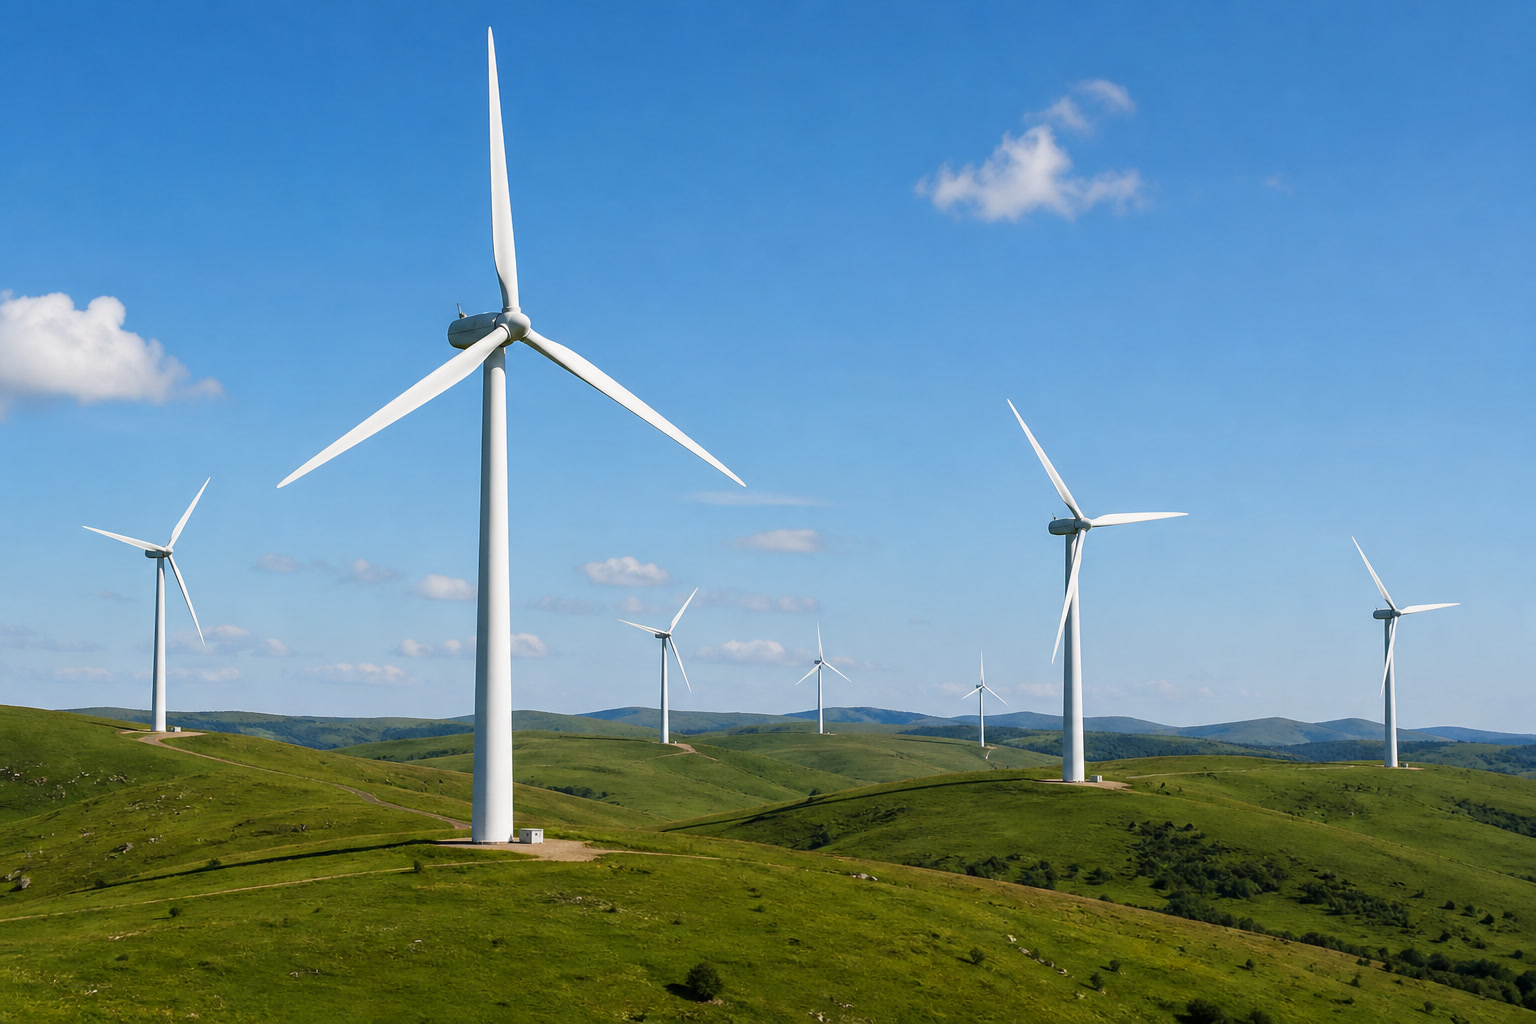
\includegraphics[width=0.58\linewidth]{images/book1/ai/g5-energy-windfarm.jpg}

{\small 你在路上能看见的一条\omterm{def:g5:everyday-energy:energy}{能量}链：流动的\omterm{def:g2:air-around-us:air}{空气}使叶片转动，涡轮机把电能送入导线。}
\end{omfigure}

\section{太阳位于餐桌的上座}

\begin{example}[几乎每条链都始于太阳]\label{ex:g5:everyday-energy:sun}
沿着大多数\omterm{def:g5:everyday-energy:energy}{能量}链往回追溯，你会走到太阳。早餐呢？
植物通过捕捉阳光而生长；你吃的谷物就是罐装的阳光。
风呢？太阳使陆地受热不均，被搅动的\omterm{def:g2:air-around-us:air}{空气}便成了风，
所以连帆船也靠阳光驱动。木材呢？是树木储存的阳光。
大坝的高处之水呢？是太阳把它举起：它\omterm{def:g2:ice-water-steam:evapcond}{蒸发}了海水，
水汽在山上降下雨来。
太阳能\omterm{def:g3:first-electric-circuit:battery}{电池}板只是省去了中间环节。
\end{example}

\begin{omfigure}
\begin{tikzpicture}[scale=0.85]
  \fill[omThm] (0.9,3.2) circle (0.45);
  \foreach \a in {0,30,...,330} {
    \draw[omThm] (0.9,3.2) ++(\a:0.62) -- ++(\a:0.26);
  }
  \node[below, font=\small] at (0.9,2.5) {太阳};
  \node[draw, thick, omMeth, font=\small] (p) at (4.3,3.2) {植物};
  \node[draw, thick, omDef, font=\small] (f) at (7.2,3.2) {食物};
  \node[draw, thick, omMeth, font=\small] (m) at (9.9,3.2) {肌肉};
  \node[draw, thick, omMeth, font=\small] (w) at (4.3,1.4)
    {受热、被搅动的空气};
  \node[draw, thick, omDef, font=\small] (v) at (8.3,1.4)
    {风与帆};
  \draw[-Stealth, very thick] (1.6,3.2) -- (p);
  \draw[-Stealth, very thick] (p) -- (f);
  \draw[-Stealth, very thick] (f) -- (m);
  \draw[-Stealth, very thick] (1.35,2.75) -- (w);
  \draw[-Stealth, very thick] (w) -- (v);
\end{tikzpicture}

{\small 两条\omterm{def:g5:everyday-energy:energy}{能量}链追溯到源头：早餐与风都
始于太阳。}
\end{omfigure}

\begin{remark}[一个我们将要讲清楚的词]\label{rem:g5:everyday-energy:promise}
目前，\omterm{def:g5:everyday-energy:energy}{能量}只是一个讲得动听的故事：储存、形式、链条。它能否
被\emph{\omterm{def:g2:measuring-length:measure}{测量}}，就像用米量长度、用克量\omterm{def:g3:measuring-mass:mass}{质量}那样？可以——
\omterm{def:g5:everyday-energy:energy}{能量}有它自己的\omterm{def:g2:measuring-length:measure}{单位}和精确的核算方法，它们将在本书后面出现，
那时你已经正式学过速度和力。
你今年追踪的这些链条是地图；
数字将来会在地图上活起来。
\end{remark}

\section{练习}

\begin{exercise}[$\star$]\label{exo:g5:everyday-energy:1}
按照本章的说法，什么是\omterm{def:g5:everyday-energy:energy}{能量}？
说出四件没有\omterm{def:g5:everyday-energy:energy}{能量}就无法发生的事。
\end{exercise}

\begin{exercise}[$\star$]\label{exo:g5:everyday-energy:2}
找出储存：一只会跑动的上发条老鼠；\ 一名骑车的人；\ 
一堆篝火；\ 一条帆船；\ 一支手电筒。
\end{exercise}

\begin{exercise}[$\star$]\label{exo:g5:everyday-energy:3}
说出五种\omterm{def:g5:everyday-energy:energy}{能量}形式，
并各举一个你日常生活中的例子。
\end{exercise}

\begin{exercise}[$\star$]\label{exo:g5:everyday-energy:4}
追踪烤面包机的\omterm{def:g5:everyday-energy:energy}{能量}链，
方法同\cref{met:g5:everyday-energy:read}：储存、转换器、输出的形式。
\end{exercise}

\begin{exercise}[$\star$]\label{exo:g5:everyday-energy:5}
追踪从大坝水库到你今晚阅读台灯的\omterm{def:g5:everyday-energy:energy}{能量}链。
\end{exercise}

\begin{exercise}[$\star$]\label{exo:g5:everyday-energy:6}
手机“没电了”。究竟是什么真正用完了？那份\omterm{def:g5:everyday-energy:energy}{能量}
按\omterm{def:g5:everyday-energy:energy}{能量}链的命题，去了哪里？
\end{exercise}

\begin{exercise}[$\star$]\label{exo:g5:everyday-energy:7}
笔记本电脑使用时，为什么底部会变热？\omterm{def:g5:everyday-energy:energy}{能量}链的哪一环
正在显现？
\end{exercise}

\begin{exercise}[$\star$]\label{exo:g5:everyday-energy:8}
说明帆船靠阳光驱动，
方法是逐步向后追溯其\omterm{def:g5:everyday-energy:energy}{能量}链。
\end{exercise}

\begin{exercise}[$\star\star$]\label{exo:g5:everyday-energy:9}
一位发明家宣称有一种灯“不需要\omterm{def:g3:first-electric-circuit:battery}{电池}、不需要插头、
不需要燃料——它会永远发光”。这一宣称违背了
\cref{rem:g5:everyday-energy:nofree}中的哪一条规律？
你应该首先向这位发明家提出什么问题？
\end{exercise}

\begin{exercise}[$\star\star$]\label{exo:g5:everyday-energy:10}
一只橡胶球从肩膀高度落下，弹起的高度越来越低，
最后静止不动。莱奥说：“它的\omterm{def:g5:everyday-energy:energy}{能量}被毁灭了。”利用
\cref{prop:g5:everyday-energy:chain}为一个更好的结局辩护——
弹跳的\omterm{def:g5:everyday-energy:energy}{能量}究竟滑入了
哪种最终形式？
\end{exercise}

\begin{exercise}[$\star\star$]\label{exo:g5:everyday-energy:11}
一些房屋用黑色屋顶面板加热水；一些用阳光和弧面镜子做饭；
太阳能\omterm{def:g3:first-electric-circuit:battery}{电池}则从日光中发电。请解释“太阳能\omterm{def:g3:first-electric-circuit:battery}{电池}板只是省去了
中间环节”这句话，出自\cref{ex:g5:everyday-energy:sun}：
在太阳与柴火的温暖之间，
有哪些中间环节？
\end{exercise}
